\documentclass{shortart}

\usepackage{amsmath, amssymb, amsthm}
\usepackage{tikz}

\title{Period 3 orbits}
\author{Dexter Chua}

\tikzset{circ/.style = {fill, circle, inner sep = 0, minimum size = 3}}

\newtheorem*{thm}{Theorem}
\newtheorem*{lemma}{Lemma}

\theoremstyle{definition}
\newtheorem*{defi}{Definition}
\newtheorem*{notation}{Notation}

\begin{document}
Suppose we are given a continuous function $f: [0, 1] \to [0, 1]$. For example, the graph of $f$ may look like this:

\begin{center}
  \begin{tikzpicture}
    \draw (0, 0) rectangle (5, 5);
    \node [left] at (0, 0) {$(0, 0)$};
    \node [right] at (5, 0) {$(1, 0)$};
    \node [left] at (0, 5) {$(0, 1)$};
    \node [right] at (5, 5) {$(1, 1)$};

    \draw [blue, semithick] (0, 0) parabola bend (2.5, 2.25) (5, 0);
  \end{tikzpicture}
\end{center}

One interesting thing to do is to randomly pick a point $x \in [0, 1]$, keep applying $f$, and see where we end up. We can visualize this process via a cobweb diagram, drawn as follows:

\begin{center}
  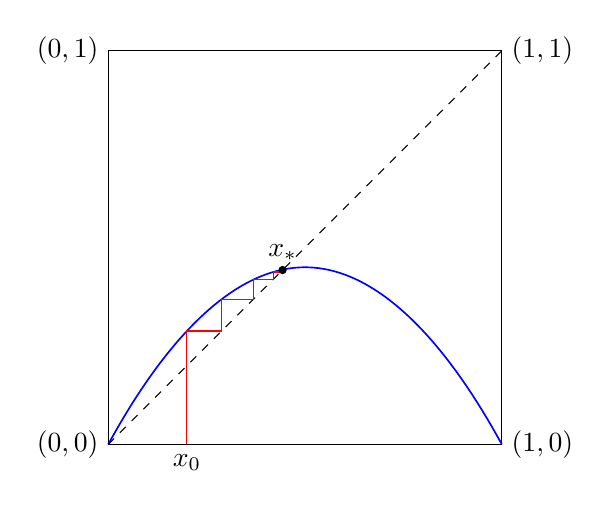
\begin{tikzpicture}
    \draw (0, 0) rectangle (5, 5);
    \node [left] at (0, 0) {$(0, 0)$};
    \node [right] at (5, 0) {$(1, 0)$};
    \node [left] at (0, 5) {$(0, 1)$};
    \node [right] at (5, 5) {$(1, 1)$};

    \draw [blue, semithick] (0, 0) parabola bend (2.5, 2.25) (5, 0);

    \draw [dashed] (0, 0) -- (5, 5);

    \draw [red] (1.0, 0) node [below, black] {$x_0$}
    -- (1.0, 1.44) -- (1.44, 1.44)
    -- (1.44, 1.845) -- (1.845, 1.845)
    -- (1.845, 2.095) -- (2.095, 2.095)
    -- (2.095, 2.19) -- (2.19, 2.19)
    -- (2.19, 2.215) -- (2.215, 2.215);

    \node [fill, circle, inner sep=0, minimum size=3] at (2.215, 2.215) {};
    \node [above] at (2.215, 2.215) {$x_*$};
  \end{tikzpicture}
\end{center}

We see that we converge towards the point $x_*$. In particular, if we start at $x_*$, we stay there all the time --- $x_*$ is a \emph{fixed point}.

Some choices of $f$ give more complicated behaviour. For example, in the following diagram
\begin{center}
  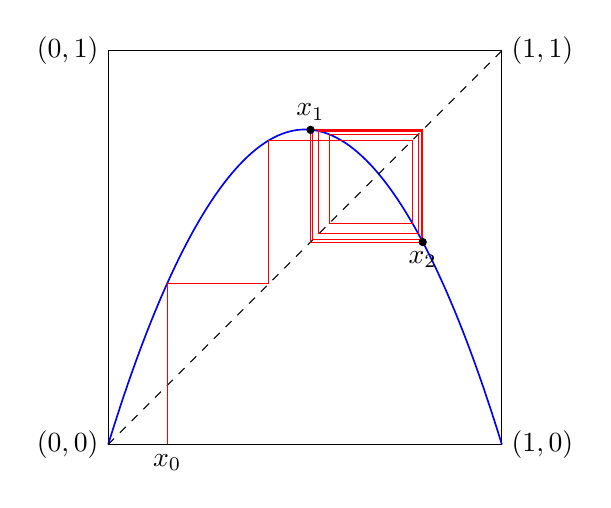
\begin{tikzpicture}
    \draw (0, 0) rectangle (5, 5);
    \node [left] at (0, 0) {$(0, 0)$};
    \node [right] at (5, 0) {$(1, 0)$};
    \node [left] at (0, 5) {$(0, 1)$};
    \node [right] at (5, 5) {$(1, 1)$};

    \draw [blue, semithick] (0, 0) parabola bend (2.5, 4) (5, 0);

    \draw [dashed] (0, 0) -- (5, 5);

    \draw [red] (0.75, 0) node [below, black] {$x_0$}
    -- (0.75, 2.04) -- (2.04, 2.04)
    -- (2.04, 3.865) -- (3.865, 3.865)
    -- (3.865, 2.81) -- (2.81, 2.81)
    -- (2.81, 3.94) -- (3.94, 3.94)
    -- (3.94, 2.675) -- (2.675, 2.675)
    -- (2.675, 3.98) -- (3.98, 3.98)
    -- (3.98, 2.6) -- (2.6, 2.6)
    -- (2.6, 3.995) -- (3.995, 3.995)
    -- (3.995, 2.57) -- (2.57, 2.57)
    -- (2.57, 3.995) -- (3.995, 3.995)
    -- (3.995, 2.57) -- (2.57, 2.57)
    -- (2.57, 3.995) -- (3.995, 3.995)
    -- (3.995, 2.57) -- (2.57, 2.57)
    -- (2.57, 3.995) -- (3.995, 3.995)
    -- (3.995, 2.57) -- (2.57, 2.57)
    -- (2.57, 3.995) -- (3.995, 3.995)
    -- (3.995, 2.57) -- (2.57, 2.57);

    \node [fill, circle, inner sep=0, minimum size=3] at (2.57, 3.995) {};
    \node [above] at (2.57, 3.995) {$x_1$};
    \node [fill, circle, inner sep=0, minimum size=3] at (3.995, 2.57) {};
    \node [below] at (3.995, 2.57) {$x_2$};
  \end{tikzpicture}
\end{center}
we see that in the limit, the point oscillates between $x_1$ and $x_2$. In this case, $x_1$ and $x_2$ are $2$-periodic points. Perhaps if we want to care about the limiting behaviour, we should understand these periodic points.

\begin{defi}
  Let $f: [0, 1] \to [0, 1]$ be a function. A point $x \in [0, 1]$ is \emph{$n$-periodic} if $f^n(x) = x$ and $f^k(x) \neq x$ for $0 < k < n$.
\end{defi}

For example, for the following choice of $f$, we have a $3$-periodic point:

\begin{center}
  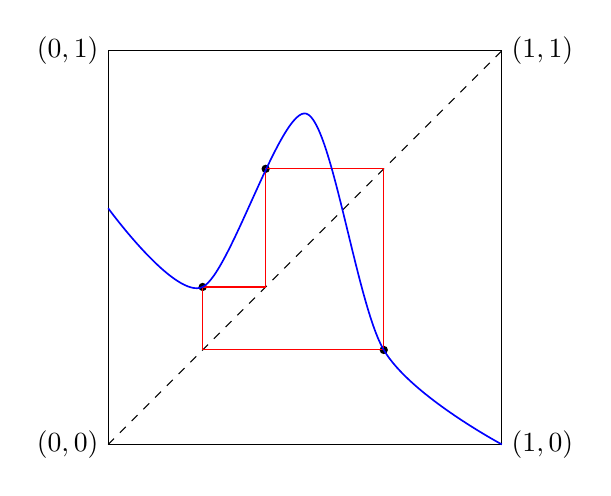
\begin{tikzpicture}
    \draw (0, 0) rectangle (5, 5);
    \node [left] at (0, 0) {$(0, 0)$};
    \node [right] at (5, 0) {$(1, 0)$};
    \node [left] at (0, 5) {$(0, 1)$};
    \node [right] at (5, 5) {$(1, 1)$};
    \draw [dashed] (0, 0) -- (5, 5);

    \node [fill, circle, inner sep=0, minimum size=3] at (1.2, 2) {};
    \node [fill, circle, inner sep=0, minimum size=3] at (2, 3.5) {};
    \node [fill, circle, inner sep=0, minimum size=3] at (3.5, 1.2) {};

    \draw [red] (1.2, 1.2) -- (1.2, 2) -- (2, 2) -- (2, 3.5) -- (3.5, 3.5) -- (3.5, 1.2) -- (1.2, 1.2);

    \draw [blue, semithick] plot [smooth] coordinates { (0, 3) (1.2, 2) (2.52, 4.2) (3.5, 1.2) (5, 0)};
  \end{tikzpicture}
\end{center}

We are now ready to state the desired theorem.

\begin{thm}
  Let $f: [0, 1] \to [0, 1]$ be a continuous function. If $f$ has a $3$-periodic point, then $f$ has an $n$-periodic point for all $n$.
\end{thm}

Let's try to understand this. A good start might be to find a fixed point, i.e.\ a $1$-periodic point. We can achieve this using the intermediate value theorem. From now on, we fix a single continuous function $f$.

\begin{lemma}
  Let $I \subseteq [0, 1]$ be a (closed) subinterval. If $f(I) \supseteq I$, then $I$ contains a fixed point.
\end{lemma}

\begin{proof}
  Write $I = [a, b]$. Then since $f(I) \supseteq I$, we in particular have $a, b \in f(I)$. So we can find $a', b' \in I = [a, b]$ such that $f(a') = a$ and $f(b') = b$. Then we have $f(a') - a' = a - a' \leq 0$ and $f(b') - b' = b - b' \geq 0$. Since $x \mapsto f(x) - x$ is continuous, we can find some $c$ such that $f( c ) - c= 0$, ie. $c$ is a fixed point.
\end{proof}

So we just need to find an interval $I$ such that $f(I) \supseteq I$. We suppose the three points in the $3$-periodic orbit are $x_0 < x_1 < x_2$. We may wlog assume that $f(x_0) = x_1$, $f(x_1) = x_2$ and $f(x_2) = x_0$.

\begin{center}
  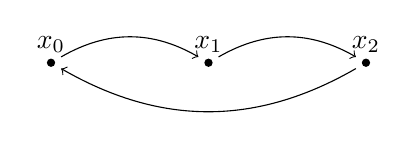
\begin{tikzpicture}
    \begin{scope}[node distance=0.5cm]
      \node [fill, circle, inner sep=0, minimum size=3] at (0, 0) {};
      \node [fill, circle, inner sep=0, minimum size=3] at (2, 0) {};
      \node [fill, circle, inner sep=0, minimum size=3] at (4, 0) {};

      \node [circle, inner sep=0, minimum size=8] (a) at (0, 0) {};
      \node [circle, inner sep=0, minimum size=8] (b) at (2, 0) {};
      \node [circle, inner sep=0, minimum size=8] (c) at (4, 0) {};

      \node [above] at (0, 0) {$x_0$};
      \node [above] at (2, 0) {$x_1$};
      \node [above] at (4, 0) {$x_2$};

      \draw (a) edge [bend left, ->] (b);
      \draw (b) edge [bend left, ->] (c);
      \draw (c) edge [bend left, ->] (a);
    \end{scope}
  \end{tikzpicture}
\end{center}

Then $f([x_1, x_2])$ is a closed subinterval containing $x_0$ and $x_2$. So it in particular contains $[x_1, x_2]$. So we have found a fixed point.

How about periodic points of larger period? If we want to find an $n$-periodic point, we might try to look for fixed points of $f^n$. This is in some sense a good strategy, but it is not good enough. If we are given a fixed point $f^n$, we know it has period \emph{at most} $n$. Perhaps it is secretly a fixed point of $f$. So we need to be a bit more delicate than that.

We first introduce a convenient notation:

\begin{notation}
  If $I, J \subseteq [0, 1]$ are subintervals, we write $I \to J$ if $f(I) \supseteq J$.
\end{notation}

We have seen that if $I \to I$, then $I$ contains a fixed point of $f$. The following is the desired strengthening of the lemma.

\begin{thm}
  If $I_0 \to I_1 \to I_2 \to \cdots \to I_{n-1} \to I_0$, then there exists an $x \in I_0$ such that $f^k(x) \in I_k$ for $k = 1, \ldots, n-1$ and $f^n(x) = x$.
\end{thm}

This is trivial if we don't require $f^k(x) \in I_k$, since $f^n(I) \supseteq I$, and we can apply the lemma. The (slightly) hard part is getting the points to lie in the $I_k$.

\begin{proof}
  Note that if $I, J \subseteq [0, 1]$ are closed subintervals with $f(I) \supseteq J$, then $f^{-1}(J)$ is a disjoint union of closed intervals contained in $I$, each of which has image $J$. By picking one of these, we get a subinterval $K \subseteq I$ such that $f(K) = J$.

  Now if $I_0 \to I_1 \to I_2 \to \cdots \to I_{n - 1} \to I_0$, then we can find some $J_{n - 1} \subseteq I_{n-1}$ such that $f(J_{n-1}) = I_0$. We still have $f(I_{n-2}) \supseteq J_{n-1}$, so we have a sequence
  \[
    I_0 \to I_1 \to I_2 \to \cdots \to I_{n-2} \to J_{n-1} \to I_0.
  \]
  We can now replace $I_{n-2}$ with a $J_{n-2}$ as above, and keep going on to obtain a new sequence
  \[
    J_0 \to J_1 \to J_2 \to \cdots \to J_{n-2} \to J_{n-1} \to I_0.
  \]
  such that $J_k \subseteq I_k$, and $f(J_k) = J_{k+1}$ for all $k$. Then since $f^n(J_0) = I_0 \supseteq J_0$, it follows that we can find some $x \in J_0$ such that $f^n(x) = x$. By assumption, $f^k(x) \in J_k \subseteq I_k$. So we are done.
\end{proof}

We are essentially done with the proof. We set $I_1 = [x_0, x_1]$ and $I_2 = [x_1, x_2]$. Then we have $I_2 \to I_2$, $I_1 \to I_2$ and $I_2 \to I_1$. If we feel like drawing diagrams, we can draw it as

\begin{center}
  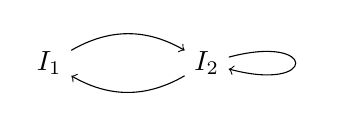
\begin{tikzpicture}
    \node (a) at (0, 0) {$I_1$};
    \node (b) at (2, 0) {$I_2$};

    \draw (a) edge [bend left, ->] (b);
    \draw (b) edge [bend left, ->] (a);

    \draw (b) edge [loop right, ->, looseness=20] (b);
  \end{tikzpicture}
\end{center}

Now we have a sequence of the form
\[
  I_1 \to I_2 \to I_2 \to \cdots \to I_2 \to I_1
\]
for any number of copies of $I_2$. So for each $n$, we get some $x \in I_1$ such that $f^n(x) = x$, and crucially, $f^k(x) \in I_2$ for all $0 < k < n$. To see that $x$ is actually of period $n$, we need to check that $f^k(x) \not= x$ for $0 < k < n$. To do so, we simply have to note that $I_1 \cap I_2  = \{x_1\}$. Thus if $f^k(x) = x$ for some $k$, then $x$ must be $x_1$. We can check manually that $x_1$ does not satisfy the required property, since $f^2(x_1) = x_0 \not\in I_2$. This concludes the proof.

This result is a special case of a more general theorem called \href{https://en.wikipedia.org/wiki/Sharkovskii\%27s_theorem}{Sharkovskii's theorem}. The statement is as follows:

\begin{thm}
  Define an ordering on the naturals by
  \[
    \begin{array}{cccccccc}
      3 &\rhd& 5 &\rhd& 7 &\rhd& \cdots &\rhd\\\\ 2\cdot 3 &\rhd& 2 \cdot 5 & \rhd & 2 \cdot 7 & \rhd & \cdots & \rhd\\\\ 2^2\cdot 3 &\rhd& 2^2 \cdot 5 & \rhd & 2^2 \cdot 7 & \rhd & \cdots & \rhd\\\\ \vdots & & \vdots & & \vdots & & \cdots & \rhd\\\\ 2^3 & \rhd & 2^2 & \rhd & 2^1 & \rhd & 1
    \end{array}
  \]
  Then if $f: [0, 1] \to [0, 1]$ has an $n$-periodic point and $n \rhd m$, then there is an $m$-periodic point.
\end{thm}

One way to prove this is to use adapt the above strategy with some clever choices of the intervals involved.

As a concluding remark, recall that we led ourselves into looking at periodic points when we tried to understand the limiting behaviour as we keep iterating $f$. In the first two examples, the fixed point and the $2$-periodic points were \emph{stable}, namely if we start somewhere near the periodic points and keep applying $f$, the point converges towards the fixed point or cycle. In general, there is no reason to believe that the periodic points given by our theorem will be stable. This makes it slightly less interesting --- there is no way we can "naturally" discover these periodic points as we did at the beginning. We must have started at exactly the periodic point to discover the periodicity.

\end{document}
